% compile with: pdflatex -shell-escape filename.tex
\documentclass[crop,tikz,convert=pdf2svg]{standalone}
\usetikzlibrary{automata}

\tikzset{
  ->,
  >=latex,
  every state/.style={thick, fill=gray!10},
  initial text=$ $,
  node distance=3cm,
}

\begin{document}

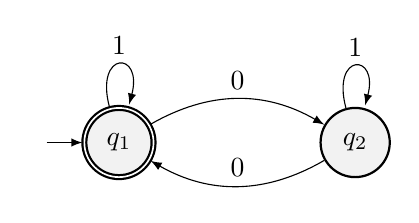
\begin{tikzpicture}
  \node[state, initial, accepting] (q1) {$q_1$};
  \node[state, right of=q1] (q2) {$q_2$};
  \draw
  (q1) edge[loop above] node{1} (q1)
  (q1) edge[bend left, above] node{0} (q2)
  (q2) edge[loop above] node{1} (q2)
  (q2) edge[bend left, above] node{0} (q1)
  ;
\end{tikzpicture}

\end{document}
